\chapter{Specification and architecture}
In order to be methodical and organized, first of all we need to specify \emph{what} exactly our project has to do. We already have some 
hints about the problem to solve, which in this section we will formalize a bit more, so now is time for the solution. Being this a 
non-trivial software we need to help us to do that with a wide angle perspective explanation of the structure we choose in order to 
successfully achieve our goals.\\
First we will deepen on the problem so we can then make an informal but concise specification of the solution based on the architecture
of the whole software project.
\section{Problem}
In \emph{sections \ref{moti}}, \emph{\ref{usecase}} and \emph{\ref{bgoals}} the problem to solve by this project is already introduced. To 
summarize it in one phrase:\\
\emph{We want our devices to automatically react to events that they can notice.}\\
This phrase sounds good as an statement, but is in fact what our devices are doing through their OS and programs, so it needs some 
further explanations. On the one hand, we must acknowledge that our solutions should give us the ability of using new kinds of events in a 
easy way for job scheduling, events we can not use for this purpose right now. On the other hand we want to centralize this job-scheduling by
noticing all the events in one program and performing actions when defined sets of these events are received. These event sets may be 
combined using logical operators, like '\emph{if noticed event\_x or event\_y then run z}'. All this should be done through the 
interface this program offers, for example a file similar to a crontab. In order to do that we also need a way to make this program notice 
any kind of events. We must remember that these events are something abstract that can represent almost everything, from a sensor detection
to an application failing. In the use case of \emph{section \ref{usecase}} we saw events like the arrival to a GPS location, an error log 
from a server and cron-like events, so the sources can be very different. We have to keep in mind that in our UNIX system there are some
hardly irreplaceable job schedulers, and we don't want to reinvent the wheel of have several job schedulers doing exactly the same. What
we expect is the ability to use the existing job schedulers to send events to our centralized system.\\
We also expressed our interest on the state-awareness of our program. It should execute an action not every time that the set of events
assigned to it are noticed, but also if a sequence of actions has been performed before.\\
A last remark about the problem is that it includes the need of noticing and reacting not only to local events, but also to events
that happened on remote devices. In this regard we have in the use case the event on the http server that happens when an error message is
logged.
\section{Solution}
\label{sec:solution}
In the \emph{figure \ref{fig:reactordia1}} we have a sketch of the solution in architecture terms we propose to the previously explained 
problem.\\
\begin{figure}[h]
  \centering
  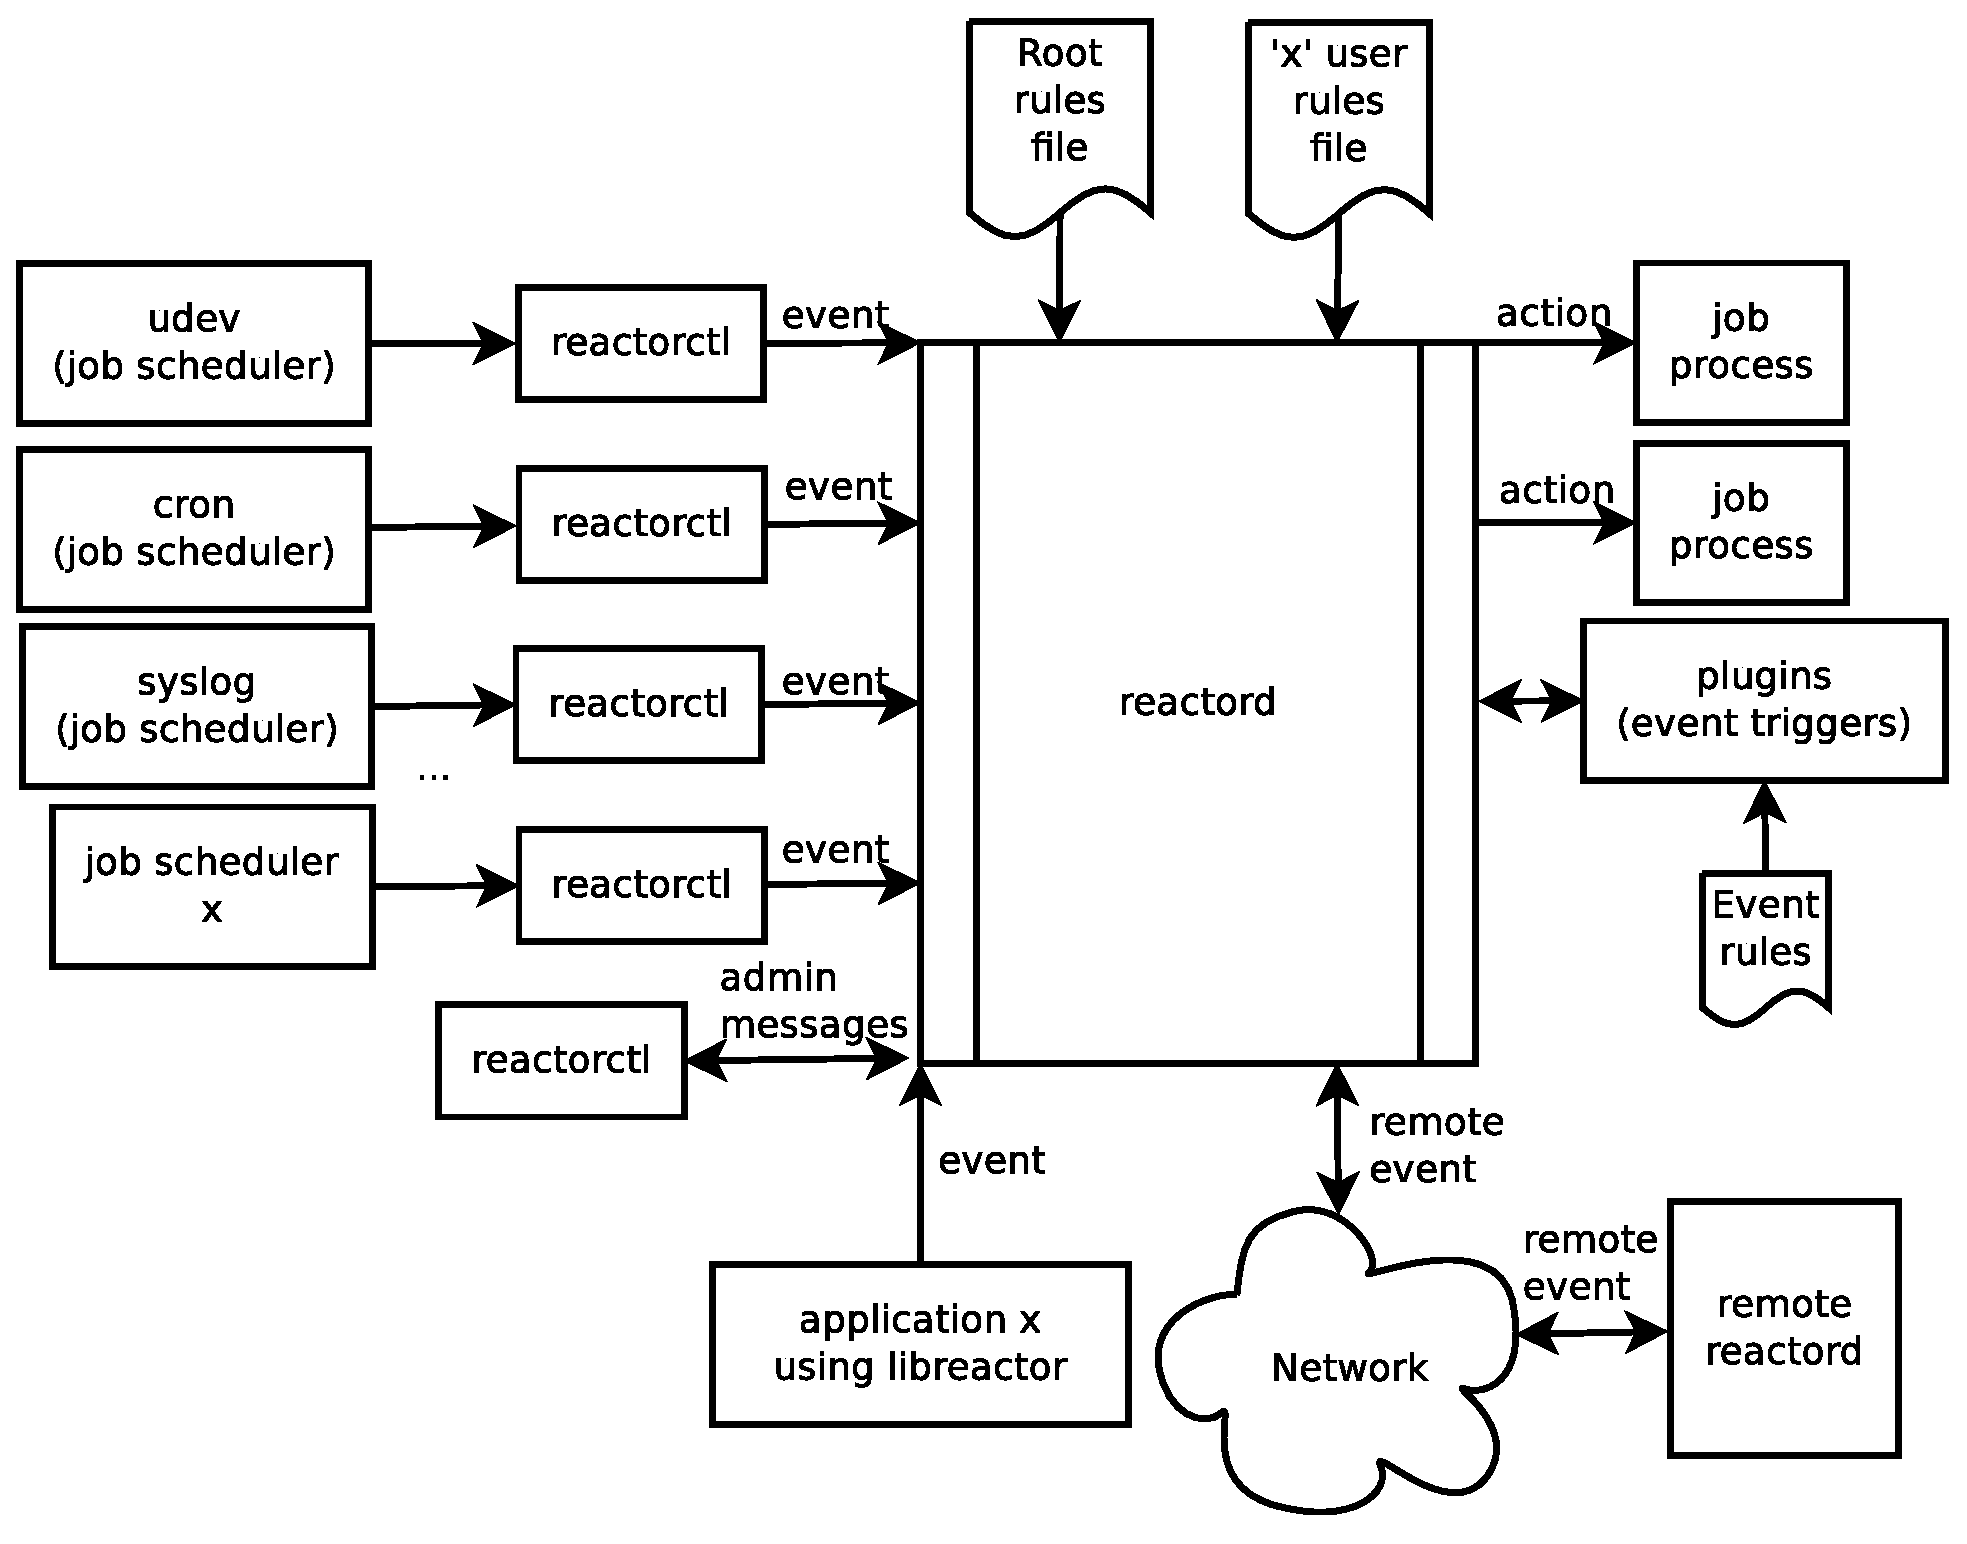
\includegraphics[width=\textwidth,keepaspectratio]{img/reactordia}
  \caption{Diagram of reactor}
  \label{fig:reactordia1}
\end{figure}

\begin{figure}[h]
  \centering
  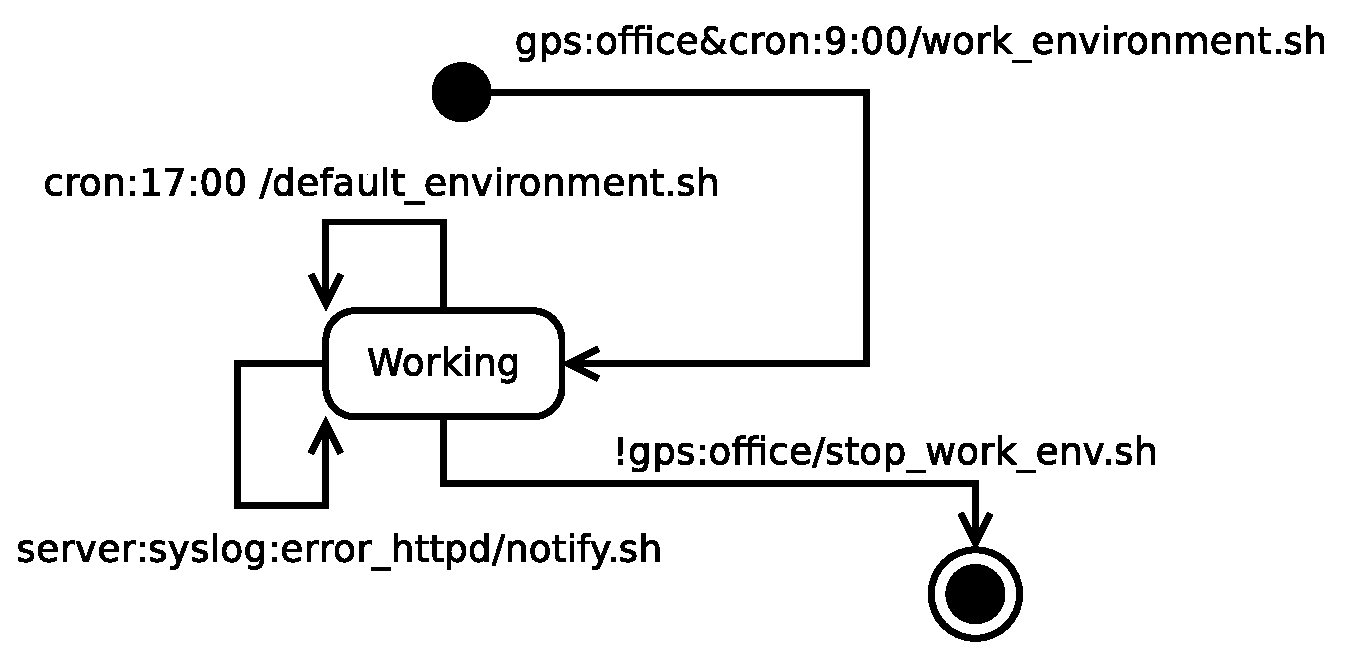
\includegraphics[scale=0.5,keepaspectratio]{img/usecasesm}
  \caption{State machine of the laptops use case}
  \label{fig:usecasesm1}
\end{figure}

\emph{reactord} is the main program, a background service, also known as daemon, that centralizes all the job scheduling. It has access
to some files called in the figure ``rules files''. The rules files are the crontab-like files where the sequence of sets of events 
assigned to actions are defined by the user. Every set of rules assigned to an action will be called a \emph{rule}. As we said before we
need some kind of state awareness with this rules, so the best we found to achieve that is by making the rules define a deterministic 
state machine. To illustrate that concept in \emph{figure \ref{fig:usecasesm1}} we can see the deterministic state machine of the web 
developers laptop use case. On the transitions between states be have the 'events/action' conjunction, where 'events' is a set of events
using the AND (\texttt{\&}) logical operator between them. This means that the transition will only be triggered when all the events are
noticed. To perform an OR operator, so an action is executed if event 'x' or event 'y' are notices, is easy with this system. The only
thing we have to do, as shown in the \emph{figure \ref{fig:exsm1}}, is define a transition between the same states with the same action 
for each OR operand. 
\begin{wrapfigure}{r}{0.5\textwidth}
  \vspace{-20pt}
  \begin{center}
    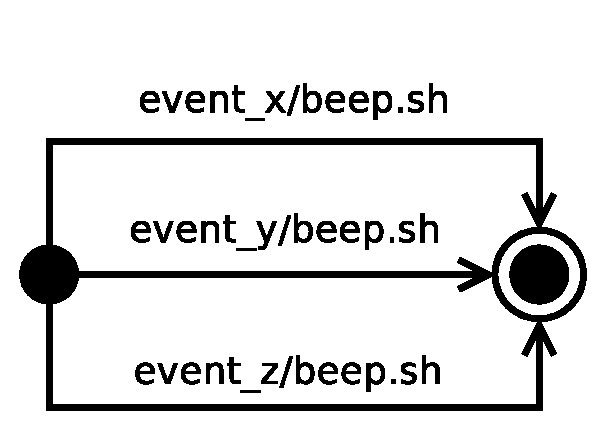
\includegraphics[scale=0.5,keepaspectratio]{img/exsm1}
  \end{center}
  \caption{Example \emph{reactord} state machine for ``run beep.sh if event\_x OR event\_y OR event\_z are noticed''}
  \label{fig:exsm1}
\end{wrapfigure}
We said that the state machines are deterministic, that means that we can have several transitions from the same state
waiting for the same events to notice. If the user defines an indeterministic state machine, it will go through one of the transitions. 
Which one it will choose is an undefined behaviour. The syntax of these rules files is defined on \emph{\ref{sec:rparser}}.\\

\emph{reactorctl} is a daemon control program that acts as a command-line interface of the daemon.
\begin{list}{-}{Its options are:}
  \item Add rule
    \subitem Unlike adding rules through the rules file, those transitions will be active at once without need of restarting the 
      daemon. Also, when the daemon is restarted the rules added with that method will disappear. The rule syntax will be the same as in
      the rules files.
  \item Send event
    \subitem It sends to the main daemon the specified event identification.
  \item Delete transition
    \subitem It deletes the specified transitions and all the dependant transitions and states of the state machine. An example is drawn 
      in \emph{figure \ref{fig:exsm2}}, where we can see how 'delete transition' not only deletes the target transition, the only one out 
      from the 'Second' state, but also all the transitions depending on it. It is important to see in the example that if we simply
      follow the transitions beginning from the transition we want to delete in order to delete them, the result state machine would be 
      empty. From the 'Third' state we go to the initial state which would be deleted, so then all the state machine would also be deleted.
      But an initial state does not depend on any transition more than the transitions out from it, so we keep it as it is expected.\\
      As in the 'add rule' option, when a transition is deleted the change will be effective instantly, but 
      if the deleted transition is from a rules file, when \emph{reactord} is restarted that transition will be restored.
\end{list}
\begin{figure}[h]
 \centering
 \begin{subfigure}[b]{0.3\textwidth}
  \centering
  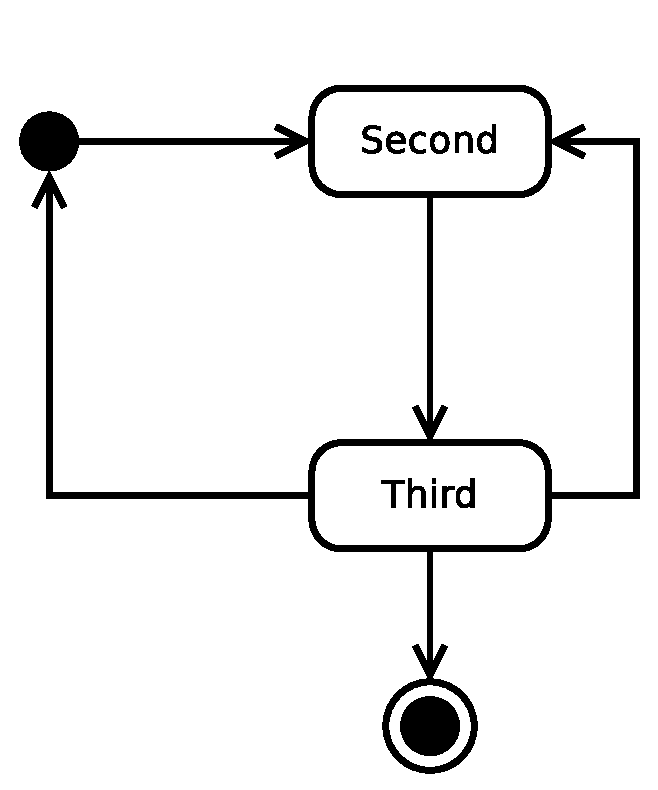
\includegraphics[width=\textwidth,keepaspectratio]{img/exsm2-1}
  \caption{Before}
 \end{subfigure}
 ~
 \begin{subfigure}[b]{0.3\textwidth}
  \centering
  \includegraphics[width=\textwidth,keepaspectratio]{img/exsm2-2}
  \caption{After}
 \end{subfigure}
 \caption{Example of a transition deletion. The deleted transition is the only one out from the 'Second' state, so 'Second' becomes final.
 The initial state and the transitions from it are kept on the result because it does not depend on its entering states.}
 \label{fig:exsm2}
\end{figure}
The 'send event' option needs special attention. Apparently there is not much use for this option than for debugging \emph{reactor},
or testing the state machines. But it is in fact an option of great use. Its main purpose is to let external, independent and already 
existing job schedulers to propagate their events to \emph{reactord}. The use is simple, \emph{reactorctl} gives us a command to send 
events that we just have to put as a command action to those existing job schedulers, let's say for example \emph{cron}:\\
\begin{center}
  \texttt{1 0 {*} {*} {*}  reactorctl -e cron\_event\_1}\\
\end{center}
With that entry in a crontab, cron will send an event called 'cron\_event\_1' to \emph{reactord} every night at 00:01.\\
And this can be used as well on other programs that are not mainly job schedulers, but do the job too and will be on our system
we like it or not (and we do). Programs like \emph{udev} or \emph{syslog} have the ability of scheduling jobs and they are critic for the 
operating system, so reimplementing its functionality just for the sake of our project won't be very smart of us. That pretty much solves 
the 'reinventing the wheel' problem. This solution can also be seen in the \emph{figure \ref{fig:reactordia1}} schema.\\
\\
These functionalities of the \emph{reactorctl} program are isolated in a shared library called \emph{libreactor}. This means that new 
programs, or plugins of a program can be built with the ability of sending events directly to \emph{reactord} whenever it finds an event 
occurred (including internal program events). That is a juicy potential source of events, because probably developers will not make their
new programs with our project in mind, but if we are interested in a program with a plugin interface to send events to \emph{reactor}, 
we can make a plugin to do so. And this is a great range of useful programs: Linux modules, Firefox, Thunderbird, Eclipse, LibreOffice...
This is not the only use of \emph{libreactor}. We also put here functions initially thought for the \emph{reactord} internals but that
actually are useful for the plugins. For example in the sketch we can easily see that both \emph{reactord} and the plugins have rule files,
son in both cases we need a rule parser that we may share. As you can imagine, the parser can't be exactly the same. This will be explained
in detail in \emph{section \ref{sec:lib}}\\
\\
In the schema we can see two sources of events more. One is \emph{reactord} itself running in a remote device. \emph{reactord} has several
kinds of actions to perform, not only command line executions. One of them is called \emph{propagate}, and what it does is send all the
event identifications that triggered the action to an specified address (which can be local, but it is quite useless). Those actions won't
be propagated in any specified order, neither in the order of arrivals nor in the order in which they were written.\\
% TODO Maybe this should be changed (in the code), so every time an event is received, it is propagated at once, instead of waiting for all
% the events to arrive, and then propagate them unsorted.
So for example in our use case, the http server should have our software installed. Then, the syslog should have a rule to execute 
\emph{reactorctl} to send an event to its \emph{reactord}. The last step would be set a \emph{reactor} rule that propagates this event to 
an IP, maybe a broadcast for a subnet dedicated to developers and sysadmins where our web developer is.\\
\\
The other sources of events left in the schema are the \emph{reactord} plugins. Their initial purpose is to to trigger new kind of events 
to the system in the easiest way possible. \emph{reactord} and \emph{libreactor} compound a set of tools and interfaces that makes 
it easy to build a plugin. By now, their behaviour is not expected to be very different from the standalone job schedulers using 
\emph{reactorctl}. Plugins will have their own rules files with their own syntax were it will be stated when an event should be triggered. 
This can be improved a lot, by for example letting use this rules directly on the \emph{reactord} rules file, or letting us ask the plugin
for an event. On \emph{section \ref{sec:future}} we will discuss future and more interesting functionalities.
% TODO Goals?
% \section{Goals}
% % TODO Extract goals from the report and extend them
\section{State of the art}
We are not alone and we are not the only ones who thought about the problem we are trying to solve, or at least similar ones. There are
existing projects with similar purposes that have been around for some years, and are quite popular. We are going to explain why, even 
existing these good projects, ours is still needed for our purposes.\\
The project we are going to comment will be event driven job schedulers and similar projects that gave us ideas and have some approaches
to our solution. We won't spend time explaining every job scheduler that exist, because this would take the whole report. The are a lot 
of job schedulers with a lot of different purposes, specially workload and calendar driven job schedulers, so in this field we will talk 
only about the event driven ones.
% TODO Section summary. Explain main general reasons to develop reactor, and why not simply use one of the existent projects.
% TODO Maybe the next sections could be subsections of types of programs, like 'Job Schedulers', 'Event Mangers', and such.
\subsection{SOS JobScheduler}
\emph{SOS JobScheduler}\cite{sos:js} is probably the most similar project to \emph{reactor}. It is an open source general purpose job 
scheduler which is mainly used to launch executable files and run database processes automatically. Has been written mainly in C++ and 
Java, its available for HP-UX(IA), IBM AIX, Linux, Solaris and Windows(2003/2008/XP/Vista/7) and it is licensed under GPL. 
It is also event driven, but its events
are different from ours. Its events are called 'job starts', so an event is just that, an order to run a job sent by somebody. It 
internally detects two kind of events that are actually noticed by well known job scheduling capable programs, so it' reinventing the
wheel. Those events are calendar and directory monitoring events, which are currently managed by \emph{cron} and \emph{at} for the first 
kind and \emph{inotify-tools} for the second one\footnote{We are obviously talking about UNIX, probably Windows has its own similar 
services.}. It also has a library to build applications that can start jobs, a user interface with the capability for sending 'job starts'
and 'job start' notification via IP.\\
The main difference with our project then is that it doesn't use state machines in order to execute its jobs. In \emph{reactord}, noticing
an event doesn't imply that an action is going to be launched. If this event is expected it will forward the state machines so it will be
nearer to run an action. Instead, in \emph{SOS JobScheduler} they don't have states but 'job chains'. A job chain is a sorted sequence of 
jobs launched by a single 'job start'. This sequence can have parallel jobs and dependencies between them. So it doesn't solve our problem,
as it doesn't require a sorted execution of jobs, but a state driven execution of them.\\
However, it has features to take into account that would be easy to develop for our project as plugins, like web service integration 
(receiving events from web services) or the timeslots. Timeslots are time periods in which the jobs should be executed. In \emph
{section \ref{sec:future}} we explain our state machine oriented solution, which is not limited to time intervals.
\subsection{Proprietary event driven job schedulers}
We believe that being able to modify the code of the project to make it solve your specific needs, and being able to receive improvements
on the software from unknown people interested on the project are two critical points that our solution must have. That's why we will 
acknowledge the proprietary job schedulers that we know in this section, they lack the same main requisite, being FLOSS.\\
\\
Global ECS is a job scheduler by Vinzant Software that offers the following features\cite{vin:gecs}:
\begin{list}{-}
    \item Single point-of-control for monitoring and managing enterprise-wide job streams.
    \item Controller/Agent model uses the power of TCP/IP to simplify communications in a distributed enterprise environment.
    \item Global ECS has many capabilities that allow for a ‘Management by Exception’ approach to automating your production environment.
    \item Multiple Method Scheduling (MMS) allows for simple programming and management of tasks with widely varying repetition schedules.
    \item Role based security model.
    \item Launches and controls any command line, including graphical and text programs, batch files, command files and macros.
    \item Captures return codes to detect job success or failure and allow the system to take appropriate actions.
    \item Controls sequential execution and branching with sophisticated job dependencies.
    \item Full support for file and resource dependencies.
    \item GECS System Events to assist in scheduling and monitoring the production environment.
    \item Full featured browser-based client for remote console access.
\end{list}
As we can see it is very focused on monitoring, and it does nothing about state machines.\\
\\
Cronacle and SAP Central Process Scheduling are job schedulers developed by Redwood. According to Wikipedia\cite{wp:rws}:
\begin{quote}
 \emph{	
    ``Cronacle is an event driven business and enterprise process automation solution. It was developed by Redwood Software in 1993 
    and is based on the use of business events to drive IT workload rather than more traditional time date based scheduling. Cronacle 
    also supports a series of extensions for specific purposes, one of which, Insight, was introduced in 2011 as a business process 
    monitor.''
  }
\end{quote}

\begin{quote}
  \emph{	
    ``The SAP Central Process Scheduling application by Redwood delivers adaptive, real-time, event-driven job scheduling and 
    process-automation capabilities. This product is sold by SAP AG.''
  }
\end{quote}
It is hard to get technical information about this projects on their companies web sites, and we are not really that interested on it. So
we will just move forward, and take into account the features they claim to have.
\subsection{udev}
\begin{quote}
  \emph{
    ``udev is the device manager for the Linux kernel. Primarily, it manages device nodes in /dev. It is the successor of devfs and 
    hotplug, which means that it handles the /dev directory and all user space actions when adding/removing devices, including firmware 
    load.''\cite{wp:udev}
  }
\end{quote}
Although \emph{udev} is not a job scheduler, as we already said, it has job scheduler capabilities. Also it uses a similar architecture to
the one that we use. The project core is the \emph{udevd} daemon process which receives administration orders from the \emph{udevadm}
command line program, and 'uevents' from the kernel. These uevents are a kind of event sent through a netlink socket that informs about
a device added or removed from the system. It has a library to make your application gain some \emph{udev} functionalities and files were 
the user and the software distributions should write rules stating how the system must react to an uevent.\\
As all the other projects it lacks the state machine running capability, and it only reacts to 'uevents'. So its clearly far from resolving
our situation by itself. But instead of that, it is a great source of inspiration for our project. \emph{udev} is a long-term project 
developed by experienced programmers and very close to the Linux kernel. We got a lot of ideas about the architecture of \emph{reactord} 
from their code and solved some design issues as well.
